\chapter{Software-Entwicklung}
Aus den anfänglichen Ideen für die Umsetzung des Lighthouse Keeper entstehen in diesem Kapitel die ersten Module für dessen Verwirklichung. Zum Anfang wird die verwendete Hardware vorgestellt und in Verbindung dazu, die Aufgaben der genutzten Software-Komponenten näher erläutert. Durch die geeignete Wahl aller Bestandteile, lassen sich viele Aufgaben auf vorgefertigten Module übertragen. Beispielsweise werden statt einer eigenen Entwicklung, ein bestehendes Kommunikations-Framework und eine bereits existierende Middleware für den Roboter genutzt. Mit der Nutzung dieser fertigen Lösungen wird im großen Maße Arbeitsaufwand eingespart und ermöglicht einen stärkeren Fokus auf das eigentliche Thema. Da dies im Hinblick auf die Smartphone-Applikation nicht immer möglich war, wird deren Implementierung in diesem Kapitel exemplarisch einmal dargestellt. 
\section{Verwendete Hardware}
Da die Beacon-Technologie vorrangig zur Indoor-Lokalisierung von Personen eingesetzt wird und als Peripheriegerät meistens ein Smartphone Verwendung findet, wird auch ein solches für die gesamte Testdauer als Messgerät genutzt. Die Wahl fiel dabei auf ein Android-Smartphone mit dem Namen Motorola Moto G der gleichnamigen Firma Motorola Inc. Es wurde ausgewählt, weil es alle Hardware- und Software-Anforderungen zum Empfang von BLE-Signalen erfüllt und als ein Standard-Smartphone gilt, sodass sich mit den ihm erzielten Ergebnisse auch auf andere Produkte übertragen lässt. Desweiteren werden zwei Roboter in den Experimenten genutzt, um die Messungen reproduzierbar und standardisiert durchzuführen. Für die reinen Distanz-Signalstärke-Messungen wird der Roboters bzw. lediglich sein Arm namens "`Youbot"' der Kuka AG und später für die Validierung einer Beacon-Konfiguration der Roboter "`Scitos G5"' der MetraLabs GmbH verwendet. 
\subsection{Motorola Moto G}
Das Moto G dient als Empfangsstation der BLE-Signale, dessen grundlegende Spezifikationen ein 1,2 GHz Snapdragon 400 Prozessor mit 1 GB RAM und ein WCN3620 BT/FM/WLAN RF Modul aussmachen (\cite{Moto}). Seine Abmaße betragen 129.9 mm $\times$ 65.9 mm $\times$ 11.6  mm bei einem Gewicht von 143 g. Desweiteren verwendet es standardmäßig ein Android 4.3 als Betriebssystem, welches jedoch für die Experimente auf die Version 4.4 geupdated wurde. Neben der technischen Austattung und Software sind für die späteren Messungen die Antennen und deren Charakteristiken von hoher Bedeutung, denn deren Eigenschaften wirken sich direkt auf den Empfang der Signale aus. Um die Einflüsse besser zu verstehen, sind in den Abbildungen \ref{fig:MotoGV} und \ref{fig:MotoA} die Anordnung der Antennen einmal skizziert. Dabei fällt es auf, dass sich WLAN- und Bluetooth-Modul die selben Antennen teilen. Dies führt zu der Frage, ob es zu Konflikten in der Funktionsweise des Smartphones kommt, wenn gleichzeitig auf beide Module zugegriffen wird. Jedoch dazu mehr im Abschnitt der App-Entwicklung. Die zweite Frage die sich daraus stellt, ist die Veränderung der Empfangs- und Sendequalität des Moto G in verschiedenen Positionen. Eine Antenne hat je nach Bauform und Funktionsweise Bereiche, in der sie mit voller leistung sendet und empfängt, aber auch Bereiche in der Funk-Signale sie weder verlassen noch erreichen können. 
\begin{figure}[b!]
$\begin{minipage}[b]{7cm}
\centering
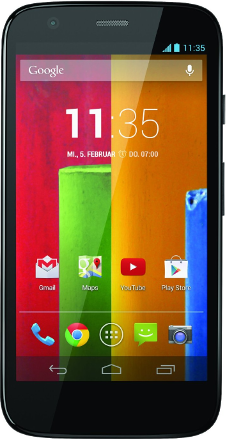
\includegraphics[width=0.45\textwidth]{Bilder/MotoG} 
\caption{Vorderseite des Motorola Moto G \cite{MotoGV}}
\label{fig:MotoGV}
\end{minipage}
\hfill
\begin{minipage}[b]{7cm}
\centering
\begin{tikzpicture}
\node [anchor=south west,inner sep=0] at (0,0) {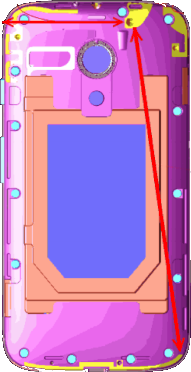
\includegraphics[width=0.45\textwidth]{Bilder/MotorolaAntenne}};
\draw [red,-angle 60,line width=0.49mm] (2.4,5.77) -- (3.375,5.77);
\node (1) at (3.375,5.77) {};
\node [right=0.1cm of 1,inner sep=0, text width = 4cm] {Bluetooth- und WLAN-Antennen};
\end{tikzpicture}
\caption{Rückseite vom Moto G mit Antennen-Gerüst  \cite{Moto}}
\label{fig:MotoA}
\end{minipage}$
\end{figure}
Das hat verschiedene physikalische Gründe, jedoch sind diesen komplexen nichtlinearen Eigenschaften der Antennen des Moto G zumindest nicht öffentlich bekannt und können auch nicht einfach bestimmt werden. Es sei nur anzumerken, dass bei den Messungen auch darauf geachtet werden muss, wie und an welchen Halte-Punkten das Moto G am besten befestigt wird, ohne deren Transceiver-Fähigkeiten negativ zu beeinflussen. Eine gute Annahme dabei ist es das Smartphone so auszurichten, als ob es flach in der Hand eines Menschen liegen würde. Der Hersteller wird schließlich darauf bedacht sein, sein Produkt für einen normalen Betrieb auszulegen und somit auch die Konstruktion und Bau der Antennen danach optimieren. Diese Annahme muss jedoch noch anhand von Messungen verifiziert werden.
\subsection{Youbot}\label{sec:You}
In vorigen Abschnitt wurde schon angesprochen, dass die Lageposition des Messinstrumentes zu seiner Empfangsleistung überprüft werden muss. Zudem soll das Smartphone so gehalten werden, als wenn es sich in einer flachen Hand befindet und so auch die Experimente durchgeführt werden. Um all dies zu erreichen und auch unter der Anforderung an einen automatisierten und reproduzierbaren Prozess, empfiehlt es sich einen Roboterarm als Mess-Plattform zu benutzen. Aufgrund der Verfügbarkeit wurde das Modell "`Youbot"' der Firma "`Kuka"' gewählt und für die Messungen mit einer Halterung aus einem 3D-Drucker regänzt (siehe Abbildung \ref{fig:Youbot1}). Die Vorteile des Systems sind zum einen der montierte hochpräzise Roboterarm mit Greifer auf dem Youbot und zum anderen, dass ein vollwertiger Rechner mit einem Linux Betriebssytem und eine drahtlose WLAN-Schnittstelle im System verbaut sind und so die Kommunikation zum Roboter sehr einfach aufgebaut werden kann. Der künstliche Arm kann sich dabei um seine fünf Achsen drehen (siehe Abbildung \ref{fig:Youbot2}) und bietet somit genug Möglichkeiten, die Lageposition vom Moto G zu verändern. 
\begin{figure}[H] 
$\begin{minipage}[b]{7cm}
\centering
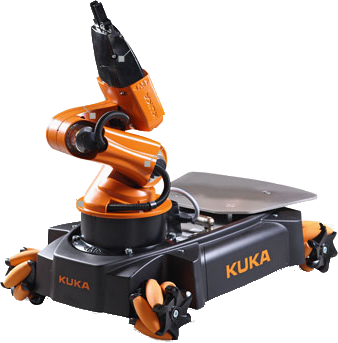
\includegraphics[scale=0.07]{Bilder/Youbot}
\caption{Youbot mit Halterung (gelber Aufsatz)}
\label{fig:Youbot1}
\end{minipage}
\hfill
\begin{minipage}[b]{8cm}
\centering
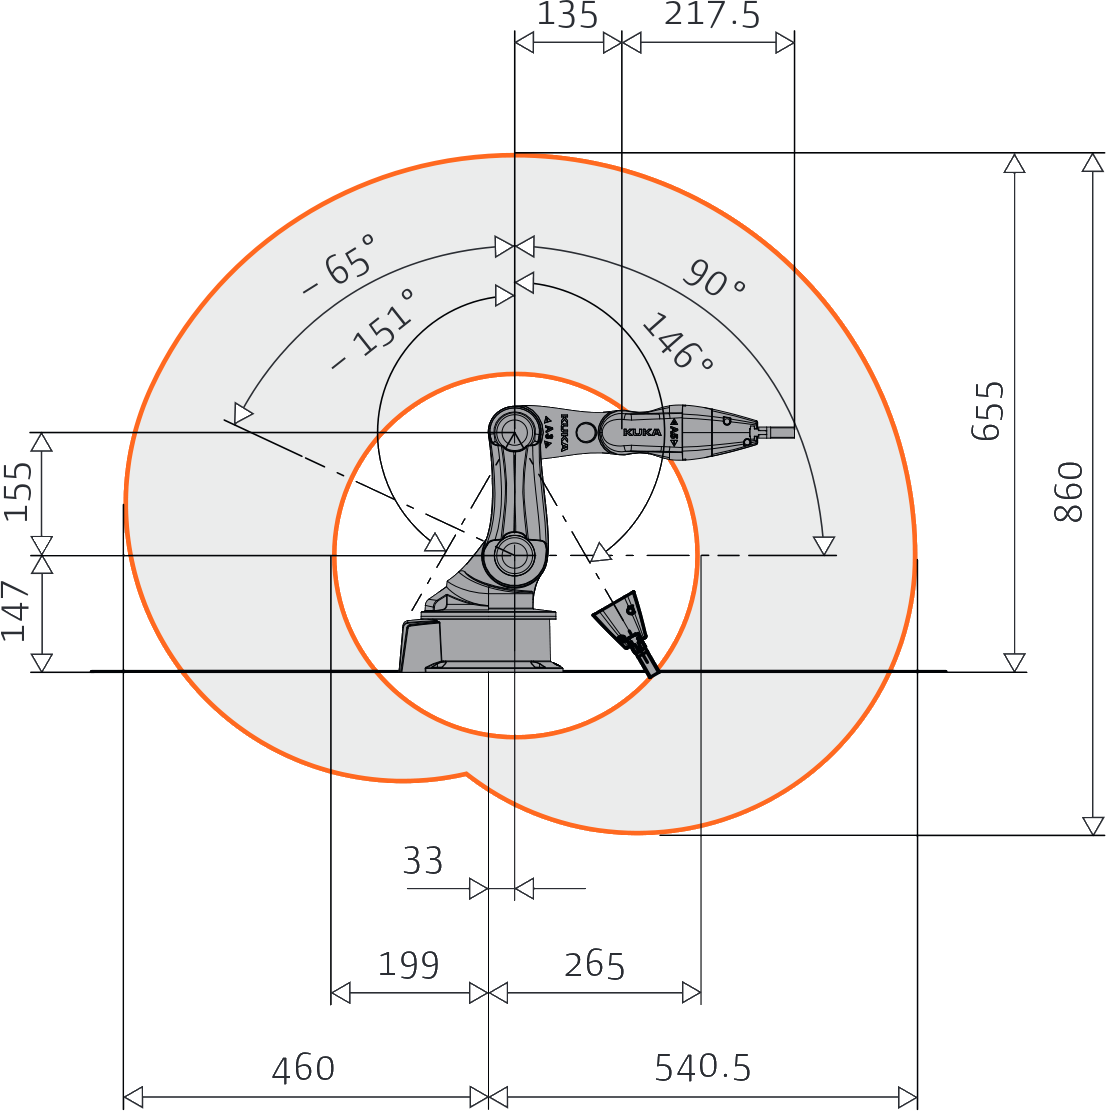
\includegraphics[scale=0.2]{Bilder/AxesYB}
\caption{Zeichnung eines Youbot-Arms und seiner fünf Rotationsachsen \cite{You}}
\label{fig:Youbot2}
\end{minipage}$
\end{figure}
\subsection{Scitos G5}
Die Durchführung der Evaluation einer Beacon-Konfiguration wäre grundsätzlich auch mit dem modifizierten Youbot aus Abschnitt \ref{sec:You} möglich. Jedoch wurde es in der Aufgabenstellung gefordert, den Roboter "`Scitos G5"' von der MetraLabs GmbH zu verwenden. Der Scitos G5 ist mit den Maßen 55 cm $\times$ 60 cm $\times$ 60 cm etwas größer als der Youbot und durch seinen Dreirad-Lenkung weniger wendig (vgl. Abbildung \ref{fig:Scitos}). Die Vorteile gegenüber dem Youbot bestechen jedoch durch seine bessere Ausstattung und den größeren Software-Umfang, weswegen es keiner zusätzlichen Entwicklungen bedarf und somit den Arbeitsaufwand für das Lighthouse Keeper-Konzept verringert wird. Der Scitos G5 verfügt über Schrittmotoren, einem Laserscanner und Inertialsensoren zur Navigation und er besitzt zudem einen leistungsfähigen Intel Core i7-Prozessor, WLAN und ein Linux-Betriebssystem, sodass auch hier genug Ressourcen für eine Kommunikation vorhanden sind. Die Machbarkeit des gesamten Kontroll-Prozesses von Beacon-Konfigurationen beruht dabei auf der Leistungsfähigkeit von diesem Roboter, denn er muss in der Lage sein, seine Position unabhängig von der Trilateration von Beacon-Signalen zu bestimmen und diese als Referenzquelle zur Verfügung zu stellen. Für seine Positionsbestimmung verwendet er die Software-Umgebung "`Miracenter"' (siehe \ref{sec:Mira} im nächsten Absatz), welche die Sensordaten aus der Wahrnehmung (Motoren, IMU, Laserscanner) so verwertet, dass sie eine Karte der Umgebung erstellen kann und somit im Abgleich von Sensorinformationen und Karte der Roboter stets seine Position kennt. Der Hersteller wirbt dabei mit einer Nutzlast von bis zu 50 kg und einer Maximalgeschwindigkeit von 1,4 $\frac{m}{s}$ bei einer batteriebetriebenen Laufzeit von ca. 20 Stunden \cite{Mira}, sodass ein künstlicher Roboterarm auf dem Scitos G5 ebenfalls denkbar wäre und somit auch die Aufgaben vom Youbot zukünftig übernimmt.
\begin{figure}[H] 
\centering
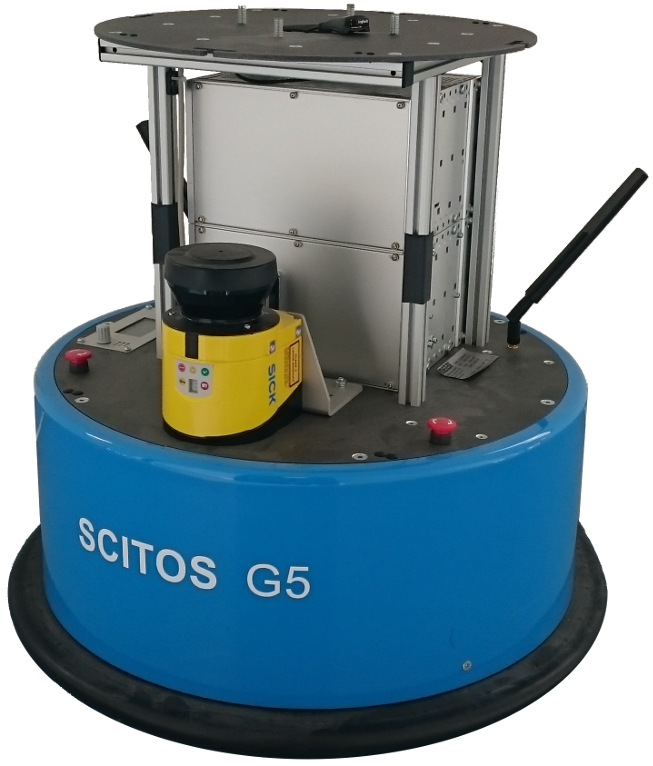
\includegraphics[scale=0.2]{Bilder/Scitos}
\caption{Scitos G5 von der MetraLabs GmbH}
\label{fig:Scitos}
\end{figure}
\section{Verwendete Software}
Um die Hardware zu nutzen und das geplante Konzept umzusetzen, benötigt es einer Kommunikation zwischen den Geräten und weiterer Werkzeuge zur Aufnahme von Messungen und deren Verarbeitung. Bei der Umsetzung wurde besonders auf Konfirmität der verschiedenen Systeme und deren reibungslosen Zusammenspiels geachtet. Um eine gemeinsame Basis zu schaffen, wurde das Software-Framework "`Robots Operating System"'(ROS) verwendet. Mit einem gemeinsamen Standard lassen sich die Messungen besser vergleichen, wodurch ihre Qualität und Aussagekraft zunimmt. Die Messungen müssen dabei auf der Smartphone-Plattform und den Roboter-Plattformen aufgenommen und  diese synchronisiert werden. Während ROS die übergeordnete Schnittstelle darstellt, müssen auf den einzelnen Hardware-Elementen die Messungen eigenständig durchgeführt werden. Die Messung auf dem Scitos-Roboter entfällt dabei auf die Software "`Miracenter"' und funktioniert ohne weiteres. Die Software für die Messungen auf dem Smartphone ist hingegen nicht vorgefertig und muss mithilfe eines Editors für Android-Applikationen und einer speziellen Bibliothek für die Kommunikation Smartphone $\leftrightarrow$ Estimote Beacon entwickelt werden.
\subsection{Robot Operating System -- ROS}
Das "`Robot Operating System"' oder kurz ROS, ist ein Projekt zur Schaffung eines flexiblen Frameworks für die Entwicklung von Software für Roboter. Daraus entstand eine der mächtigsten Sammlungen aus Werkzeugen, Bibliotheken und Normen, um komplexes Verhalten zwischen Robotern über verschiedenste Robotik-Plattformen robust zu gestalten \cite{ROSErkl}. Der Anwendungsbereich für ROS ist demzufolge sehr umfangreich, jedoch werden für diese Arbeit nur folgende Eigenschaften \cite{ROSPaper} des Projektes benötigt und hier näher betrachtet:
\begin{itemize}
\item "`Peer to Peer"' (P2P)-Verbindungen
\item Modularem Aufbau
\item Unterstützung mehrerer Programmiersprachen
\item freier Nutzung und Open-Source
\end{itemize}
Das Kommunikation-Framework des Lighthouse Keeper-Konzeptes, welches auf ROS aufbaut, besteht dabei aus mehreren miteinander verbundenen Rechnern (sog. "`Hosts"') die zur Laufzeit über P2P miteinander kommunizieren. Bei der P2P-Verbindung können alle Teilnehmer ihre Dienste bzw. ihre Informationen gleichermaßen einander anbieten und nutzen, indem sie Daten im Netzwerk gleichzeitig empfangen und senden können. Dabei läuft auf einem zentralen Server der eigentliche Kern des Frameworks, über den der sämtliche Datenverkehr geleitet wird. Und auf den Host-Systemen laufen die eigentlichen modularen Anwendungen ("`Nodes"'), die über Schnittstellen ("`Sockets"') des Betriebssytems ihre Daten auf das Netzwerk und schließlich an ROS verteilen. Dadurch können die Nodes in verschiedenen Sprachen programmiert werden, die lediglich auf die entsprechende Schnittstelle zugreifen. Ausgehend von den Nodes werden den gesendeten Nachrichten gesondert Bezeichnungen ("`Topics"') zugeordnet und mit einem Datentyp versehen. Diese Informationen sind allen Teilnehmer des P2P-Netzwerkes bekannt und können auch von ihnen angefordert werden. Der Kern organisiert dabei eine einheitliche Uhrzeit, die dadurch für alle Nachrichten bzw. deren Zeitstempel in den verteilten Systemen konsistent bleibt und so eine Synchronisierung der Messgeräte nicht mehr nötig wird. Somit ermöglicht die Verwendung von ROS den Aufbau der gesamten Kommunikation, wie es in der Konzept-Planung in \ref{sec:KonSofArch} gefordert wurde. Zudem erleichtert ROS durch sein großen Funktionsumfang nachfolgende Erweiterungen und bietet somit Freiheiten für zukünftige Aufgaben.
\subsection{Miracenter}\label{sec:Mira}
\begin{wrapfigure}{r}{8cm}
\centering
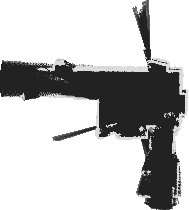
\includegraphics[scale=1.1]{Bilder/Flur}
\caption{Erstellter Grundriss eines Flures in Gebäude 29 der OvGU, Stockwerk 3}
\label{fig:Flur}
\end{wrapfigure}
Das Paket "`CogniDrive"', als Bestandteil der Software "`Miracenter"' von der Firma MetraLabs GmbH, dient als Navigator des Scitos G5 und ermöglicht es mit ihm den Grundriss eines Raumes zu erstellen (siehe Abbildung \ref{fig:Flur}) und zusätzlich die Lokalisierung des Roboters in diesem durchzuführen. Während beispielsweise der Roboter entlang der Wände fährt, messen seine Schrittmotoren den zurückgelegten Weg, die Inertailsensoren verfeinern die Informationen und erweitern sie um die Ausrichtung des Roboters. Dabei misst zusätzlich der Laserscanner die Distanz zu den Wänden und allen anderen festen Objekten in Reichweite. Aus der Fusion aller Messwerte lässt sich so der Grunsriss des vermessenden Raumes generieren. Im nebenstehendem Bild ist eine solche Karte als Beispiel aufgeführt. Die Daten die Miracenter dem Nutzer zur Verfügung stellt, bestehen dabei aus der Position des Roboters und seiner Ausrichtung in der Karte. Die Karte liegt dabei als "`Portable Network Graphics"' (PNG)-Datei vor, wobei ein Pixel einer konstanten metrischen Länge entspricht, deren Verhältnis in einer "`Extensible Markup Language"' (XML)-Datei definiert ist. Die Farbwerte der Bildpunkte beschreiben zudem, ob an einer Stelle ein Hinderniss oder ein frei befahrbarer Raum vorliegt. In der Abbildung ist zu erkennen, dass die erstellte Karte teilweise verrauscht ist, Wände nicht gerade verlaufen, oder offene Türen und herumlaufende Personen die Messungen verfälschen. Die Karte kann dafür nach der Erstellung von jedem beliebigen Bildbearbeitungsprogramm geöffnet und bearbeitet werden. Dabei ist darauf zu achten die Auflösung nicht zu verändern, da ansonsten die Dimensionen nicht mehr übereinstimmen oder gegebenenfalls die XML-Datei anpasst werden. Nach der Bearbeitung der Bilddatei kann sie anschließend im Miracenter geladen werden. Mittels Mausklick in die Karte wird die ungefähre Position des Roboters bestimmt. Danach orientiert sich der Scitos G5 automatisch und lokalisiert sich im weiteren Verlauf selbst anhand seiner Sensordaten. Nun können ihm Positionen und Ausrichtung vorgegeben werden und durch seiner internen Pfadplanung steuert er sie autonom an. Durch ein Miracenter-ROS-Interface kann dabei die interne Lokalisierung und die Vorgabe von Position und Ausrichtung vom Scitos extern übermittelt werden. Die gesamte Software ist jedoch proprietär, d.h. nicht quelloffen, sodass ein tieferer Blick in die Funktionsweise der Software hier verwehrt wird.
\subsection{Android-Studio, Estimote SDK und ROSjava}\label{sec:Hilfen}
Als letzten Baustein in der Software-Architektur fehlt die App für das Moto G, deren Entwicklung auf dem Zusammenwirken dreier Grundpfeiler aufgebaut sein wird:
\begin{enumerate}
\item Das Android-Studio \cite{AndStu} ist eine Entwicklungsumgebung für Programme speziell von Android-Smartphones. Es bietet die  Mittel eine Applikation, basierend auf der Programmiersprache Java, auf ein Android-Gerät zu portieren und dort auch zu testen. Aufgrund der Implementierung der "`Integrated Development Environment"' (IDE) in Java, lässt es sich auf beinahe jedem Betriebssystem verwenden und bietet dadurch eine hohe Flexibilität in der Anwendung.
\item Damit die Applikation die Beacon-Signale verarbeiten kann, müssen die gesendeten Nachrichtenpakete und das verwendete BLE-Protokoll in das Programm eingebettet werden. Vom Hersteller der Beacons wird dafür eigens eine Bibliothek unter dem Namen "`Estimote Software Development Kit (SDK)"' \cite{EstSDK} bereitgestellt, die sich problemslos integrieren lässt und einfach zu bedienen ist.
\item Um die empfangenen Signale an den Server via P2P zu senden, muss eigens eine Schnittstelle von der Java-basierten Android-App zum in C/C++ gehaltenen ROS implementiert werden. Dafür wird das Paket "`Rosjava"' \cite{ROSjava} benötigt, um die Unterstützung von ROS-Funktionen für Java-Programme zu realsieren. Dies erlaubt es ROS-Pakete in eine Android-App zu integrieren und dadurch die zu übermittelnden Nachrichten-Formate darin auch zu verwenden.
\end{enumerate}
\section{App-Entwicklung}
Um das geplante Programm auf dem Smartphone zu verwirklichen, werden die aus \ref{sec:Hilfen} beschriebenen Hilfen und zudem eigener Programmcode benötigt. In diesem Abschnitt werden die einzelnen Elemente der App erläutert und ihr Zusammenspiel in der fertigen Applikation anschließend betrachtet. 
\subsection{Beacon-Detektierung}
Der kritischste, aber der auch am essentiell wichtigste Programmteil ist die Aufnahme von Beacon-Signalen. Hierfür muss die SDK von Estimote in die App über das Android-Studio als Bibliothek importiert werden. Daraufhin stehen neue Klassen und Objekte der IDE zur Verfügung, die speziell auf die Verwendung von Beacons zugeschnitten sind. Zum einen muss dabei die App bei jedem Start für die Nutzung mit Beacons mit Abfragen neu initialisiert werden, das wären zum Beispiel die Überprüfung, ob Bluetooth angeschalten ist oder ob BLE überhaupt auf dem Gerät unterstützt wird. Desweiteren muss der sogenannte Beacon-Manager, welcher im Hintergrund der App läuft, mit Zeiten für die Pause zwischen zwei Abtastungen und der Länge eines Scans, eingestellt werden. Die Problematik der Abstastraten wird hierbei später im Programmablaufplan noch erörtert. Zum anderen muss eine Art Empfangs-Funktion geschrieben werden, die bis zur Beendigung des Programms auf Meldungen der Leuchtfeuer wartet und diese für die Verarbeitung im Programm aufbereitet. Die Anwendung von Filtern oder dergleichen entfällt hier, da schließlich das Verhalten er Signalausbreitung studiert werden soll und zusätzliche Einflüsse die Ergebnisse verfälschen könnten. Interessanter wird es bei der Frage, wie häufig die Abfragen der Eingänge nach Beacon-Signalen stattfinden sollen. Hierbei stellt sich noch eine viel wichtigere Frage und zwar der nach der Funktionsweise der SDK. Also wie die Datenströme, die von den Beacons in Intervallen gesendet, darauf vom Beacon-Manager aufgenommen werden. Denn die Sende-Intervalle der Beacons können variieren, während die Applikation mit festen Werten für alle Beacons initilisiert werden muss. Die Antwort nach den Abläufen im Beacon-Manager kann leider nicht beantwortet werden, da die Entwickler keinen Einblick in ihren Quellcode gewähren und auch sonst keine Angaben oder Dokumentationen veröffentlichen. Eine bessere Veranschaulichung dieser Problematik findet sich im Abschnitt über den Programmablauf.
\subsection{Lagemessung}
Parallel zur Beacon-Detektierung soll gleichzeitig die Lage des Smartphones gemessen werden, um die Antennen-Charakteristiken besser zu verstehen und ihre Einflüsse auf die Empfangsqualität zu untersuchen. Für diese Aufgabe müssen die Inertialsensoren oder auch englisch "`Inertial Measurement Unit"' (IMU) aus Gyroskop, Beschleunigungssensor und Magnetometer vom Smartphone ausgelesen werden, was jedoch einfach umzusetzen ist, da die IDE nativ dafür Bibliotheken bereitstellt. \\ \\
Bei der Messung stellt sich hierbei die Frage nach der Häufigkeit der Sensordatenabfragen, denn letztendlich senden die Beacon -- zwar asynchron -- ihre Signale alle 2 s bis 50 ms, jedoch können die Inertialsensoren in Intervallen von mehreren hundert Hertz ausgelesen werden. Aufgrund der höheren Verfügbarkeit der IMU-Daten, wäre es jedoch nicht zwechmäßig diese permanent über das Netzwerk zu senden und somit das Datenvolumen unnötigerweise künstlich aufzublähen. Es reicht daher völlig zu jedem Zeitpunkt an dem ein Messung nach Beacon-Signalen definiert ist, eine Lageposition vom Smartphone vorrätig zu haben. Jedoch lässt sich dabei durch die schnelleren Messungen die Qualität der Informationen mit einem Filter erhöhen. Im Hinblick auf noch genügend freie Rechenkapazitäten auf dem Smartphone (bisher lediglich Abfragen der Sensoren), wurde ein Komplementärfilter auch im Hinblick auf die Sensordatenfusion von den drei IMU-Sensoren gewählt. Der dazu nötige Quellcode wurde aus \cite{IMUFilter} entnommen, der im Grunde den Drift des Gyroskops und das Signalrauschen des Beschleunigungssensors und des Magnetometers entfernt. Der Aufbau ist diesbezüglich in Abbildung \ref{fig:IMUFilter} einmal skizziert. Die gesamte Funktionsweise beruht auf dem Prinzip der Fusion mehrerer Daten, um die Qualität der eigentlichen Information zu erhöhen. Es würde für den Zweck der Orientierungserfassung des Smartphones ausreichen, die Information vom Schwerkraft-Vektors des Beschleunigungssensors mit der des Magnetometers zusammenzufassen und lediglich diese auszugeben. Jedoch sind besonders die Daten des Magnetometers sehr verrauscht, sodass ein Tiefpass oder anders ausgedrückt ein Mittelwert aus den Daten gebildet wird. Da das Moto G zusätzlich über eine Gyroskop verfügt, welches die Bewegung des Smartphones viel genauer messen kann, wird auch diese Informationsquelle benötigt. Aber auch hier existiert es ein Nachteil in dessen Anwendung. Und zwar der Drift, sprich das Aufsummieren/Integrieren der Fehler oder des Messrauschens über die Zeit. Um auch diesem Problem zu begegnen, werden die Daten nur über kleine Zeitabschnitte mithilfe eines Hochpasses gesammelt. Dadurch werden anhand der Daten aus Accelerometer und Magnetometer als Stützinformationen und die Daten vom Gyroskop als Informationen über schnelle Änderungen verwendet. 
\begin{figure}[t!]
\centering
\begin{tikzpicture}[auto, >=latex']
	\node [block2] (Accel) {Accelerometer};
	\node [block2, below=1.5cm of Accel] (Magnet) {Magnetometer};
	\node [block2, below=1.5cm of Magnet] (Gyro) {Gyroskop};
	\node [sum, right=0.8cm of Gyro] (sum1) {};
	\node [block2, below=1cm of sum1] (TS) {Zeitschritt};
	\node [draw, fill=blue!20, rectangle, rounded corners, text centered, minimum height=1.5cm, right=0.8cm of sum1] (SumZ) {$\sum$};
	\node [block2, right=1cm of SumZ] (RGyro) {Orientierung Gyroskop};
	\node [block2, right=1cm of RGyro] (HP) {Hochpassfilter};
	\node [sum, above=3.45cm of HP] (sum2) {};
	\node [block2, left=0.8cm of sum2] (TP) {Tiefpassfilter};
	\node [block2, left=1cm of TP] (RAcc) {Orientierung Accel/Magno};
	\node [block2, right=0.8cm of sum2] (LB) {Lage-\\ bestimmung};
    \draw [draw,->] (Accel.east) -- ++(1,0) -| (RAcc.north);
    \draw [draw,->] (Magnet.east) -- ++(1,0) -| (RAcc.south);
    \draw [draw,->] (RAcc) -- (TP);
    \draw [draw,->] (TP) -- (sum2);
    \draw [draw,->] (sum2) -- (LB);
    \draw [draw,->] (Gyro) -- (sum1);
    \draw [draw,->] (TS.north) -| node[pos=0.9] {$\times$} (sum1.south);
    \draw [draw,->] (sum1) -- (SumZ);
    \draw [draw,->] (SumZ) -- (RGyro);
    \draw [draw,->] (RGyro) -- (HP);
    \draw [draw,->] (HP.north) -- node[pos=0.95] {$+$} (sum2.south);
\end{tikzpicture}
\caption{Aufbau des Komplementärfilters, in Anlehnung an \cite{IMUFilter}}
\label{fig:IMUFilter}
\end{figure}
\subsection{ROS-Anbindung}
Die Realisierung der Datenübertragung über eine ROS-Schnittstelle in der App wurde so umgesetzt, dass nach dem Start der Applikation ein Feld zur manuellen Eingabe der Adresse des Servers bzw. des ROS-Masters (z.B. die Internetprotokoll (IP)-Adresse) eingegeben werden muss. Dies ist nötig, um einen Zielort für die Nachrichten zu bestimmen. Nach der manuellen Eingabe wartet der sogenannte "`Publisher"' -- also der Programmteil, der die Nachrichten aufbereitet und an das Netzwerk übermittelt -- auf die Messdaten. Dabei muss für den Publisher eine Bibliothek bereitstehen, die die Anzahl der zu übertragenden Informationen und deren Datentypen definiert und in Java integrieren kann, um sie später in der App zu verwenden. Dazu muss, wie anfänglich erwähnt die ROSjava-Erweiterung intalliert sein und anschließend das Message-Format als Java-Paket damit erstellt werden. Da die versendeten Daten schon in vorigen Abschnitten erläutert wurden, wird in Abbildung \ref{fig:ROSjavaImpl} nur noch eine Zusammenfassung in Form der Implementierung präsentiert. Das dargestellte Message-Format enthält dabei die UUID empfangener Beacons als Zeichenkette oder String-Wert, sowie der empfangenen Signalstärke RSSI und der eingestellten Sendeleistung (bezeichnet als Power), als 32 Bit Integer und der daraus errechneten Distanz als 64 Bit Flieskommazahl (ein zusätzliches Feature der Estimote SDK). Desweiteren beinhaltet sie die errechnete Orientierung vom Moto G und über allem den Zeitstempel der Zusammenstellung der Nachricht. Natürlich existiert zwischen Aufnahme der Messungen und dem Sendezeitpunkt eine zeitliche Differenz (kleiner als 1 ms Bearbeitungszeit), welche jedoch für die langsame Dynamik des Systems in den ersten Experimenten zu vernachlässigen ist. 
\begin{figure}[H]
\centering
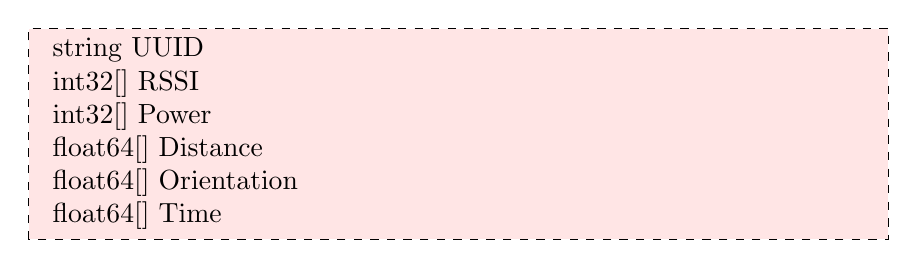
\begin{tikzpicture}
\node[rectangle, fill=red!10,minimum width=0.9\textwidth] (m) {\begin{minipage}{0.85\textwidth}string UUID\\
int32[] RSSI\\
int32[] Power\\
float64[] Distance\\
float64[] Orientation\\
float64[] Time
\end{minipage}};
\draw[dashed] (m.south west) rectangle (m.north east);
\end{tikzpicture}
\caption{Quellcode-Beispiel eines Message-Paketes für eine ROSjava-Implementierung}
\label{fig:ROSjavaImpl}
\end{figure}
\subsection{Programmablauf}
Nachdem die einzelnen Module fertig gestellt wurden, musste aus ihnen ein gesamtes Programm zusammengefügt werden. Bei der Vereinigung der einzelnen Programmteile kristallisierten sich dabei verschiedene Probleme, die unter anderem auch auf den verstärkten Einsatz von proprietärer Software zurückzuführen sind. Denn bei der notwendigen Verwendung von nicht quelloffener Software, können Fehlfunktionen der App, die eigentlich auf dem Versagen der genutzten Software beruht, lediglich umgangen oder zumindest mit Einschränkungen im Ablauf der Applikation behoben werden. Im konkreten Fall verursachte die gleichzeitige Verwendung von WLAN und Bluetooth, nach anscheinend willkürlichen Nutzungszeiten der App, Abstürze derjenigen. Das Problem scheint hierbei primär bei Android zu liegen, weil der Sachverhalt schon seit zwei Jahren in diversen Online-Foren bekannt ist, jedoch der Fehler weiterhin auch in den neuesten Versionen des Betriebssystems auftritt \cite{AndWLBT}. Der günstigste Fall den Konflikt zu lösen, wäre es einfach die Nutzung von Bluetooth durch die Estimote SDK und dem Gebrauch der WLAN-Verbindung besser zu organisieren. Jedoch bietet die SDK keine Einstellmöglichkeiten und keinerlei Dokumentation über die Verwendung des Bluetooth-Adapters, sodass auch nicht auf Seiten der WLAN-Übertragung die Anpassung stattfinden kann. Da die Zeit fehlte, sich weder mit dem Entwicklerteam der Firma Estimote auseinander zu setzen oder sich in das Android-Betriebssystem einzurbeiten, war die Lösung eher primitiv als elegant. In Abbildung \ref{fig:AppAblauf} ist die gesammte App als Ablaufplan mit Blockschaltbildern dargestellt. Während die eigntliche AUfgabe der Applikation schon im Vorfeld erklärt wurde, fällt hier eine zusätzliche Funktion, hier als Kontroll-Funktion bezeichnet, auf. Diese ist im Grunde eine Sicherheitsabfrage, wo vor der Messung und der Sendung der Nachricht über den Publisher kontrolliert wird, ob eine Verbindung zum P2P-Netzwerk existiert. Es fiehl in den unzähligen Testläufen des Programmes auf, dass sobald die WLAN-Verbindung wegbricht, der Publisher kein Ziel für seine Nachrichten ausfindig machen kann und dadurch es logischerweise zum Veragen der Funktionen führt. Durch Zuhilfenahme der Debug-Funktion vom Android-Studio konnte auch die Zeile ausfindig gemacht werden, die zum Absturz des Programmes führt. Und zwar versucht der Publisher nach der missglückten Transmission ständig auf das WLAN-Modul zuzugreifen und wenn dazu noch der Beacon-Manager versucht, den Bluetooth-Adapter bei der Detektierung zu aktivieren, geschieht der Zusammenstoß und das Programm wird außerplanmäßig beendet. Nachdem mit der Abfrage schon die Messung bei fehlender WLAN-Verbindung unterbunden wird und die Systeme erst deaktiviert und dann einzeln reaktiviert werden, lief die App durchgehend 24 Stunden ohne Vorkommnisse.   
\pgfdeclarelayer{background}
\pgfdeclarelayer{foreground}
\pgfsetlayers{background,main,foreground}
\begin{figure}[H]
\centering
\begin{tikzpicture}[auto, >=latex']
	\node [draw, fill=blue!30, rectangle, very thick, text width=2.9cm, text centered, minimum height=1.5cm] (Start) {Start};
	\node [below=0.5cm of Start] (Hilf) {};
	\node [block2, below=1cm of Start] (Eingabe) {Eingabe des ROS-Masters};
	\node [block2, below=1cm of Eingabe] (Init) {Initailisierung Beacon-Manager};
	\node [block2, below=1cm of Init] (WLAN) {WLAN-Verbinding hergestellt?};
	\node [below=0.5cm of WLAN] (Hilf2) {};
	\node [draw, fill=blue!20, diamond, text width=2cm, text centered, minimum height=1cm, below=1.5cm of WLAN] (Messung) {Messungen};
	\node [block2, left=4cm of Hilf] (BLEWLAN) {BLE/WLAN deaktivieren};
	\node [block2, below=1cm of BLEWLAN] (WLANakt) {WLAN \\ aktivieren};
	\node [below=0.5cm of WLANakt] (Hilf3) {};
	\node [block2, below=1cm of WLANakt] (WLAN2) {WLAN-Verbinding hergestellt?};
	\node [block2, below=1cm of WLAN2] (BLE) {Bluetooth aktivieren};
	\node [block2, below left=1cm of Messung] (BeaDet) {Beacon-Detektierung};
	\node [block2, below right=1cm of Messung] (Lage) {Orientierungs-Messung};
	\node [draw, fill=blue!20, diamond, text width=2cm, text centered, minimum height=1cm, below=1.5cm of Messung] (Publisher) {Publisher};
	\node [block2, below=1cm of Publisher] (Abbruch) {Programm-Abbruch?};
	\node [draw, fill=blue!30, rectangle, very thick, text width=2.9cm, text centered, minimum height=1.5cm, below=1cm of Abbruch] (Ende) {Ende};
	\draw [draw,->] (Start) -- (Eingabe);
	\draw [draw,->] (Eingabe) -- (Init);
	\draw [draw,->] (Init) -- (WLAN);
	\draw [draw,->] (WLAN) -- node[pos=0.5] {Ja} (Messung);
	\draw [draw,->] (Messung.west) -- ++(-1,0) -| (BeaDet);
	\draw [draw,->] (Messung.east) -- ++(1,0) -| (Lage);
	\draw [draw,->] (BeaDet) -- ++(0,-2) |- (Publisher.west);
	\draw [draw,->] (Lage) -- ++(0,-2) |- (Publisher.east);
	\draw [draw,->] (Publisher) -- (Abbruch);
	\draw [draw,->] (Abbruch) -- node[pos=0.5] {Ja} (Ende);
	\draw [draw,->] (WLAN.west) -- ++(-1.25,0) node[pos=0.5] {Nein} -- ++(0,8) -- ++(-1,0) -| (BLEWLAN.north);
	\draw [draw,->] (BLEWLAN) -- node[pos=0.5] {sleep}(WLANakt);
	\draw [draw,->] (WLANakt) -- node[pos=0.5] {sleep}(WLAN2);
	\draw [draw,->] (WLAN2) -- node[pos=0.5] {Ja}(BLE);
	\draw [draw,->] (BLE) -- ++(0,-1) |- node[below right] {sleep}(Messung.north);
	\draw [draw,->] (Abbruch.east) -- ++(3.5,0) node[near start] {Nein}  -- ++(0,11) |- (WLAN.east);
	\path (WLAN2) edge [loop left] node[below right=0.8cm] {Nein} node[pos=0.5] {sleep} (WLAN2);
    \begin{pgfonlayer}{background}
        \path (BLEWLAN.north -| BLEWLAN.west)+(-3.2,1.5) node (a) {};
        \path (BLE.south -| BLE.east)+(+0.5,-1.5) node (b) {};
        \path[fill=yellow!10,rounded corners, draw=black!50, dashed] (a) rectangle (b);   
    \end{pgfonlayer}	
    \node [rectangle, text width=2.9cm,below right=0.2cm of a] (Kontrolle) {Kontroll-Funktion};
\end{tikzpicture}
\caption{Programmablaufplan der Lighthouse Keeper Applikation für Android-Smartphones}
\label{fig:AppAblauf}
\end{figure}